\documentclass[20pt,]{extarticle}
\usepackage[margin=0.6in]{geometry}
\pagenumbering{gobble}
\usepackage{lmodern}
\usepackage{amssymb,amsmath}
\usepackage{ifxetex,ifluatex}
\usepackage{fixltx2e} % provides \textsubscript
\ifnum 0\ifxetex 1\fi\ifluatex 1\fi=0 % if pdftex
  \usepackage[T1]{fontenc}
  \usepackage[utf8]{inputenc}
\else % if luatex or xelatex
  \ifxetex
    \usepackage{mathspec}
  \else
    \usepackage{fontspec}
  \fi
  \defaultfontfeatures{Ligatures=TeX,Scale=MatchLowercase}
\fi
% use upquote if available, for straight quotes in verbatim environments
\IfFileExists{upquote.sty}{\usepackage{upquote}}{}
% use microtype if available
\IfFileExists{microtype.sty}{%
\usepackage{microtype}
\UseMicrotypeSet[protrusion]{basicmath} % disable protrusion for tt fonts
}{}
\usepackage{hyperref}
\PassOptionsToPackage{usenames,dvipsnames}{color} % color is loaded by hyperref
\hypersetup{unicode=true,
            pdftitle={Introduction to Locality-Sensitive Hashes},
            pdfauthor={Tyler Neylon},
            colorlinks=true,
            linkcolor=black,
            citecolor=Blue,
            urlcolor=Blue,
            breaklinks=true}
\urlstyle{same}  % don't use monospace font for urls
\usepackage{graphicx,grffile}
\makeatletter
\def\maxwidth{\ifdim\Gin@nat@width>\linewidth\linewidth\else\Gin@nat@width\fi}
\def\maxheight{\ifdim\Gin@nat@height>\textheight\textheight\else\Gin@nat@height\fi}
\makeatother
% Scale images if necessary, so that they will not overflow the page
% margins by default, and it is still possible to overwrite the defaults
% using explicit options in \includegraphics[width, height, ...]{}
\setkeys{Gin}{width=\maxwidth,height=\maxheight,keepaspectratio}
\IfFileExists{parskip.sty}{%
\usepackage{parskip}
}{% else
\setlength{\parindent}{0pt}
\setlength{\parskip}{6pt plus 2pt minus 1pt}
}
\setlength{\emergencystretch}{3em}  % prevent overfull lines
\providecommand{\tightlist}{%
  \setlength{\itemsep}{0pt}\setlength{\parskip}{0pt}}
\setcounter{secnumdepth}{5}
% Redefines (sub)paragraphs to behave more like sections
\ifx\paragraph\undefined\else
\let\oldparagraph\paragraph
\renewcommand{\paragraph}[1]{\oldparagraph{#1}\mbox{}}
\fi
\ifx\subparagraph\undefined\else
\let\oldsubparagraph\subparagraph
\renewcommand{\subparagraph}[1]{\oldsubparagraph{#1}\mbox{}}
\fi
\usepackage{subfig}
\AtBeginDocument{%
\renewcommand*\figurename{Figure}
\renewcommand*\tablename{Table}
}
\AtBeginDocument{%
\renewcommand*\listfigurename{List of Figures}
\renewcommand*\listtablename{List of Tables}
}
\usepackage{float}
\floatstyle{ruled}
\makeatletter
\@ifundefined{c@chapter}{\newfloat{codelisting}{h}{lop}}{\newfloat{codelisting}{h}{lop}[chapter]}
\makeatother
\floatname{codelisting}{Listing}
\newcommand*\listoflistings{\listof{codelisting}{List of Listings}}

\title{Introduction to Locality-Sensitive Hashes}
\author{Tyler Neylon}
\date{521.2018}

% Begin custom, non-pandoc commands.

\newcommand{\latexonlyrule}{\rule}
\newenvironment{densearray}{\begin{array}{rcl}}{\end{array}}
\newcommand{\class}[1]{}
\newcommand{\Rule}[3]{}
\newcommand{\optquad}{\quad}
\newcommand{\smallscrneg}{}
\newcommand{\smallscr}[1]{}
\newcommand{\bigscr}[1]{#1}
\newcommand{\smallscrskip}[1]{}

% End custom, non-pandoc commands.

\begin{document}
\maketitle

\newcommand{\R}{\mathbb{R}}
\newcommand{\Z}{\mathbb{Z}}
\newcommand{\eqnset}[1]{\left.\mbox{$#1$}\;\;\right\rbrace\class{postbrace}{ }}
\providecommand{\optquad}{\class{optquad}{}}
\providecommand{\smallscrneg}{\class{smallscrneg}{ }}
\providecommand{\bigscr}[1]{\class{bigscr}{#1}}
\providecommand{\smallscr}[1]{\class{smallscr}{#1}}
\providecommand{\smallscrskip}[1]{\class{smallscrskip}{\hskip #1}}

\emph{Locality-sensitive hashing} (LSH) is a set of techniques that
dramatically speed up search-for-neighbors or near-duplication detection
on data. These techniques can be used, for example, to filter out
duplicates of scraped web pages at an impressive speed, or to perform
near-constant-time lookups of nearby points from a geospatial data set.

Let's take a quick look at other types of hash functions to get a
bird's-eye view of what counts as a \emph{hash function}, and how LSH
fits into that world. A traditional use for hash functions is in
\emph{hash tables}. As a reminder, the hash functions used in a hash
table are designed to map a piece of data to an integer that can be used
to look in a particular \emph{bucket} within the hash table to retrieve
or delete that element. Many containers with string keys, such as
JavaScript objects or Python dictionaries, are based on hash tables.
Although hash tables might not \emph{guarantee} constant-time lookups,
in practice they effectively provide them.

There are other classes of hash functions as well. For example, the
\href{https://en.wikipedia.org/wiki/SHA-1}{SHA-1} cryptographic hash
function is designed to be \emph{difficult to reverse}, which is useful
if you want to store someone's password as a hashed value. Hash
functions like these are called
\href{https://en.wikipedia.org/wiki/Cryptographic_hash_function}{\emph{cryptographic
hash functions}}.

Hash functions typically have these key properties:

\begin{itemize}
\tightlist
\item
  They map some type of input, such as strings or floats, to discrete
  values, such as integers.
\item
  They're designed so that two inputs will result in hash outputs that
  are either different or the same based on key properties of the
  inputs.
\end{itemize}

Here's how LSH fits in: Locality-sensitive hash functions are
specifically designed so that hash value collisions are \emph{more
likely} for two input values that are \emph{close together}. Just as
there are different implementations of secure hash functions for
different use cases, there are different implementations of LSH
functions for different data types and for different definitions of
being \emph{close together}. In this post, I'll give a brief overview of
the key ideas behind LSH and take a look at a simple example based on an
idea called \emph{random projections}, which I'll define in section 2
below.

\section{A human example}\label{a-human-example}

It will probably be much easier to grasp the main idea with an example
you can relate to. This way we can build some intuition before diving
into those random projections that we'll use in the next section.

Suppose you have a million people from across the United States all
standing in a huge room. It's your job to get people who live close
together to stand in their own groups. Imagine how much time it would
take to walk up to each person, ask for their street address, map that
to a lat/long pair, then write code to find geographic clusters, and
walk up to every person again and tell them how to find the rest of
their cluster. I cringe just thinking about the time complexity.

Here's a much better way to solve this problem: Write every U.S. zip
code on poster boards and hang those from the ceiling. Then tell
everyone to go stand under the zip code where they live.

Voila! That's much easier, right? The main idea here is also the main
idea behind locality-sensitive hashes. We're taking an arbitrary data
type (a person, who we can think of as a ton of data including their
street address), and mapping that data into a set of discrete values
(zip codes) such that people who live close together probably hash to
the same value. In other words, the clusters (people with the same zip
code) are very likely to be groups of neighbors.

A nice benefit of the zip code approach is that it's
\emph{parallel-friendly}. Instead of requiring a center of
communication, every person can walk directly to their destination
without further coordination. This is a bit surprising in light of the
fact that the result (clusters of neighbors) is based entirely on the
\emph{relationships} between the inputs.

Another property of this example is that it is \emph{approximate}: some
people may live across the street from each other, but happen to have
different zip codes, in which case they would not be clustered together
here. As we'll see below, it's also possible for data points to be
clustered together even when they're very far apart, although a
well-designed LSH can at least give some mathematical evidence that this
will be a rare event, and some implementations manage to guarantee this
can never happen.

\section{Hashing points with
projections}\label{hashing-points-with-projections}

In this section, we'll explain exactly how a relatively straightforward
LSH approach works, explore some key parameters for this LSH system, and
review why it's an order of magnitude faster than some other approaches.

Let's start with an incredibly simple mathematical function that we can
treat as an LSH. Define \(h_1:\R^2 \to \Z\) for a point
\(x=(x_1, x_2)\in\R^2\) by

\[ h_1(x) := \lfloor x_1 \rfloor; \]

that is \(h_1(x)\) is the largest integer \(a\) for which \(a\le x_1.\)
For example, \(h_1((3.2, -1.2)) = 3.\)

Let's suppose we choose points at random by uniformly sampling from the
origin-centered circle \(\mathcal C\) with radius 4:

\[ \mathcal C := \{ (x, y) : x^2 + y^2 \le 4^2 \}. \]

Suppose we want to find which of our points in \(\mathcal C\) are close
together. We can estimate this relationship by considering points \(a\)
and \(b \in \mathcal C\) to be clustered together when
\(h_1(a) = h_1(b).\) It will be handy to introduce the notation
\(a \sim b\) to indicate that \(a\) and \(b\) are in the same cluster.
With that notation, we can write our current hash setup as

\[ a \sim b \iff h_1(a) = h_1(b). \]

Figure~\ref{fig:fig1} shows an example of such a clustering.

\begin{figure}
\centering
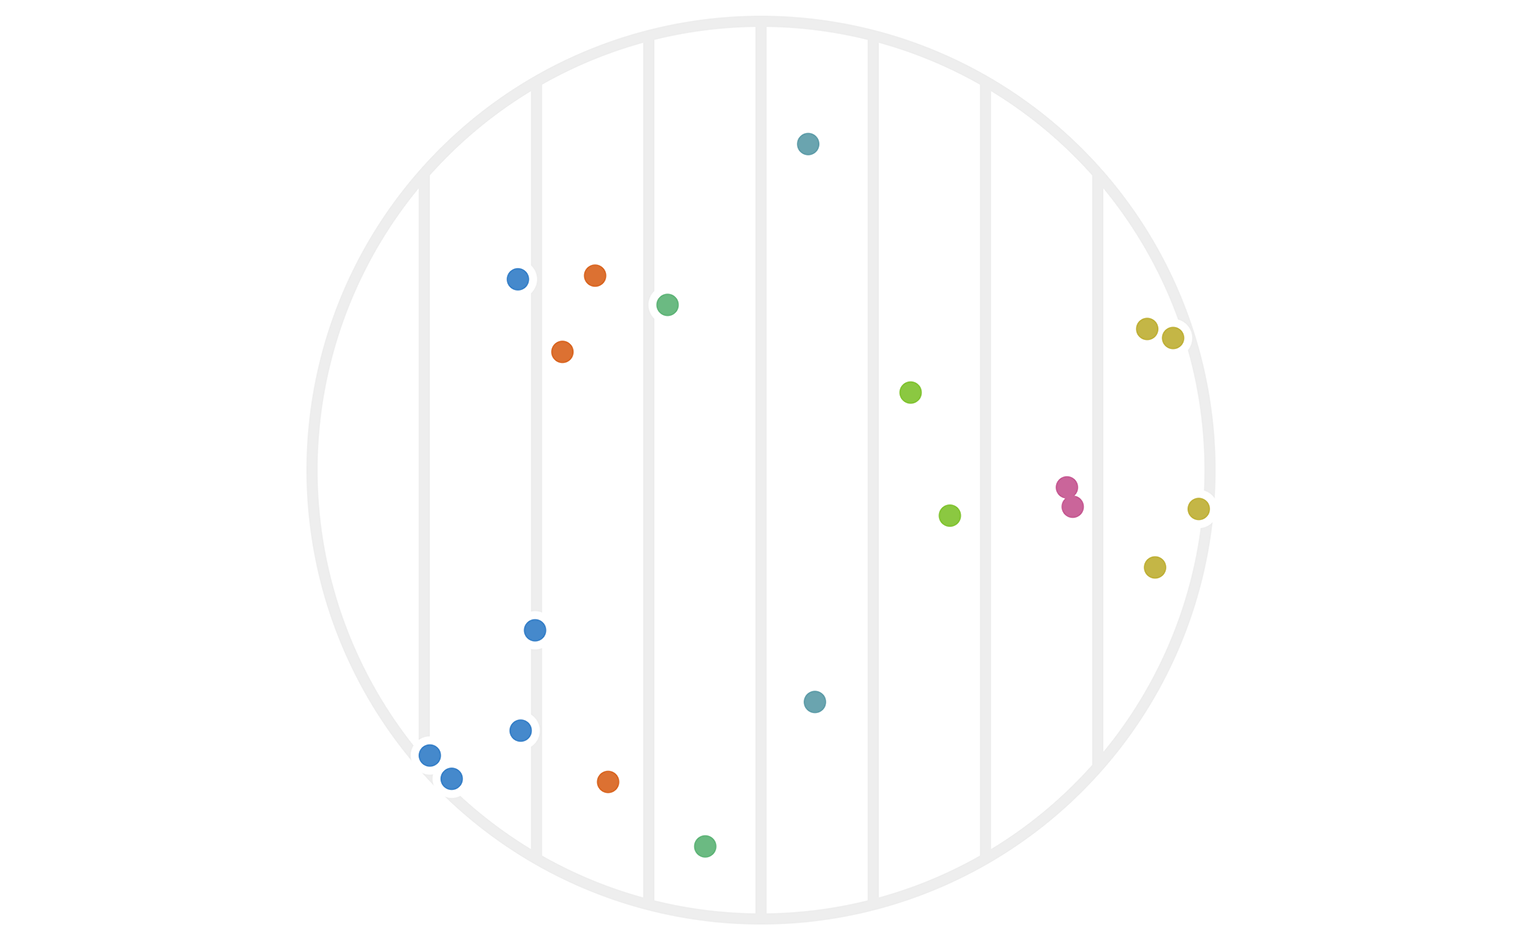
\includegraphics{images/lsh_image1_v2.png}
\caption{Twenty points chosen randomly in a circle with radius 4. Each
point \(x\) is colored based on its hash value
\(h_1(x).\)}\label{fig:fig1}
\end{figure}

You can immediately see that some points are far apart yet clustered,
while others are relatively close yet unclustered. There's also a sense
that this particular hash function \(h_1\) was arbitrarily chosen to
focus on the x-axis. What would have happened with the same data if we
had used instead \(h_2(x) := \lfloor x_2 \rfloor?\) The result is
figure~\ref{fig:fig2}.

\begin{figure}
\centering
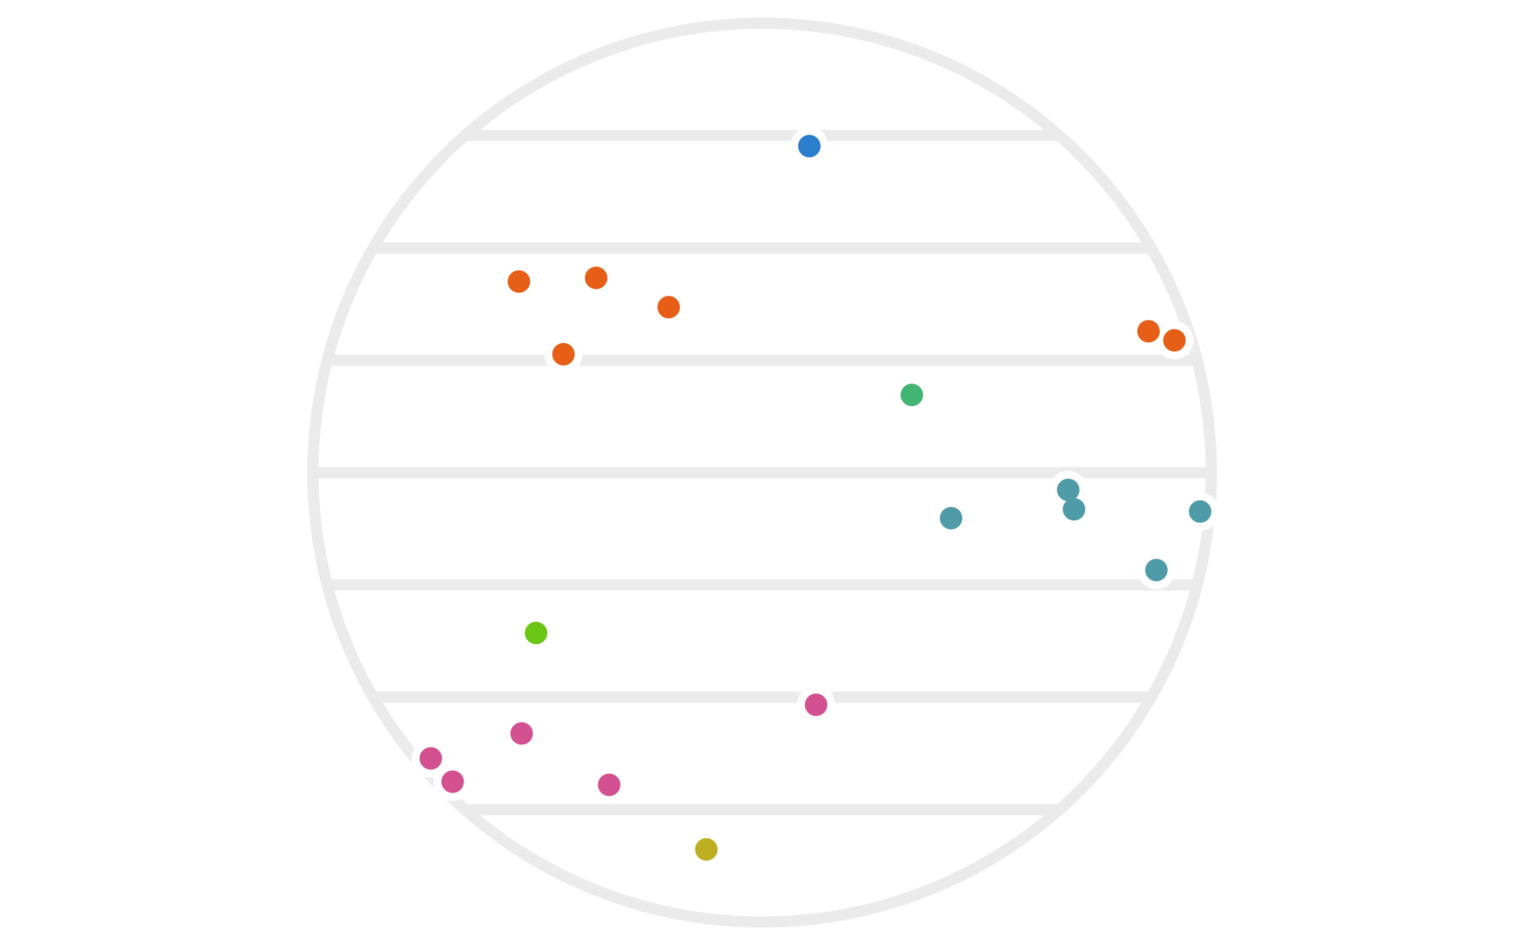
\includegraphics{images/lsh_image2.png}
\caption{The same twenty points as figure 1, except that we're using the
\(y\) values (instead of \(x\) values) to determine the hash-based
cluster colors this time around.}\label{fig:fig2}
\end{figure}

While neither clustering alone is amazing, things start to work better
if we use both of them simultaneously. That is, we can redefine our
clustering via

\begin{equation} a \sim b \iff h_1(a) = h_1(b) \text{ and } h_2(a) = h_2(b). \label{eq:eq1}\end{equation}

Our same example points are shown under this new clustering in
figure~\ref{fig:fig3}.

\begin{figure}
\centering
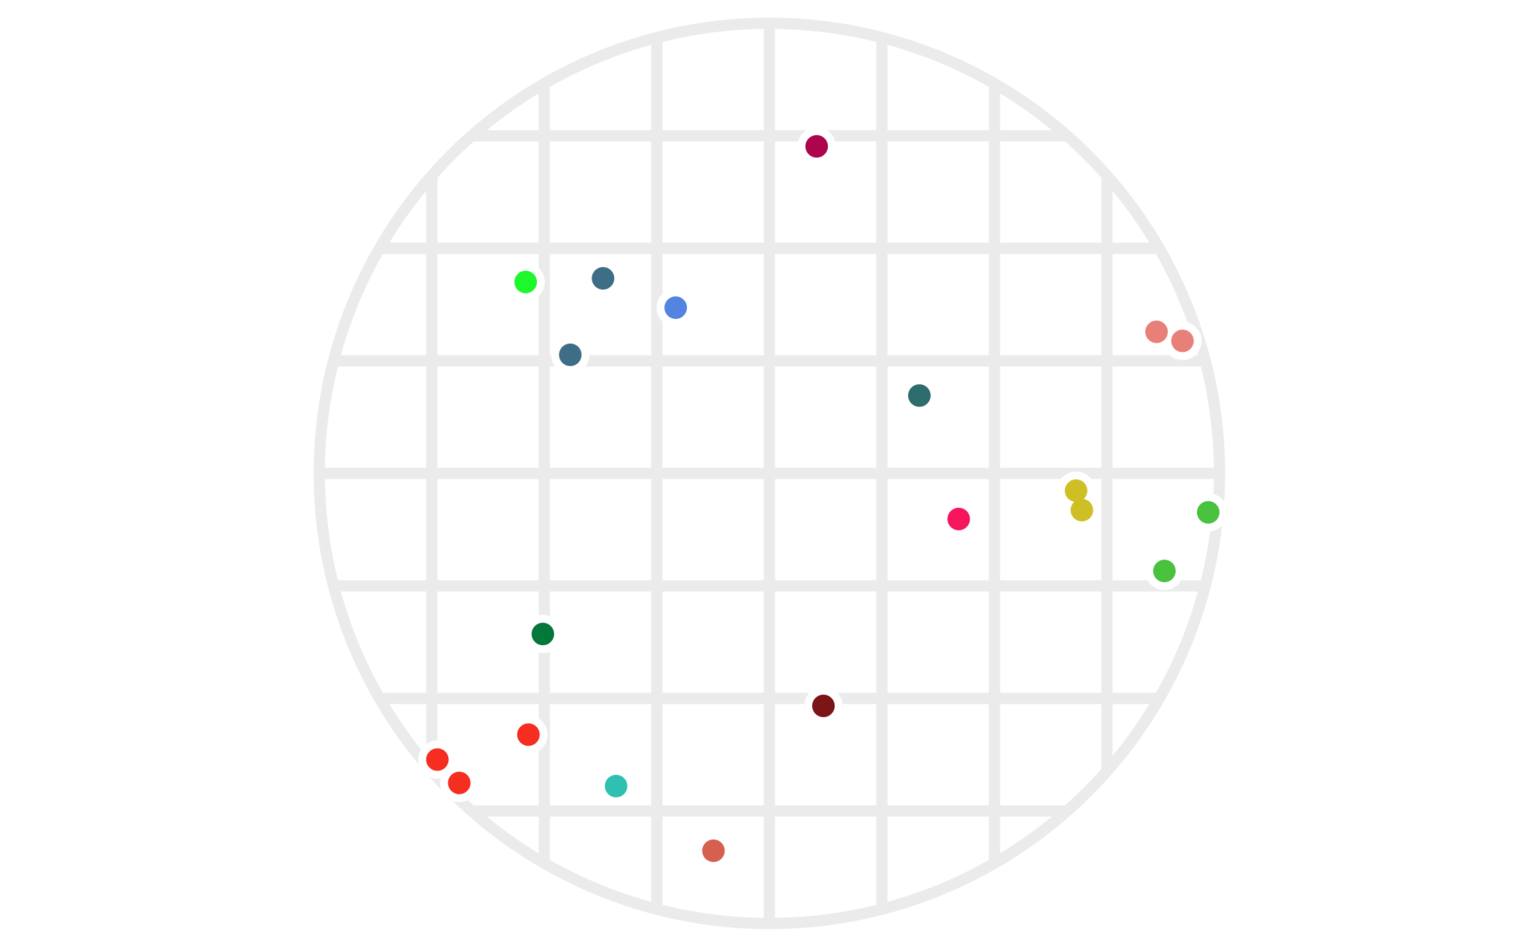
\includegraphics{images/lsh_image3.png}
\caption{The same twenty points clustered via two different hashes ---
one using \(\lfloor x\rfloor\), the other using \(\lfloor y\rfloor.\) As
before, points are colored based on which cluster they're in; a cluster
is the set of all points who share both their \(\lfloor x\rfloor\) and
their \(\lfloor y\rfloor\) values.}\label{fig:fig3}
\end{figure}

This does a much better job of avoiding clusters with points far apart,
although, as we'll see below, we can still make some improvements.

\subsection{Randomizing our hashes}\label{randomizing-our-hashes}

So far we've defined deterministic hash functions. Let's change that by
choosing a random rotation matrix \(U\) (a rotation around the origin)
along with a random offset \(b \in [0, 1).\) Given such a random \(U\)
and \(b,\) we could define a new hash function via

\[ h(x) := \lfloor (Ux)_1 + b \rfloor, \]

where I'm using the notation \(( \textit{vec} )_1\) to indicate the
first coordinate of the vector value \emph{vec}. (That is, the notation
\((Ux)_1\) means the first coordinate of the vector \(Ux\).)

It may seem a tad arbitrary to use only the first coordinate here rather
than any other, but the fact that we're taking a random rotation first
means that we have the same set of possibilities, with the same
probability distribution, as we would when pulling out any other single
coordinate value.

The advantage of using randomized hash functions is that any theoretical
properties we want to discuss will apply without having to worry about
pathologically weird data. Conceptually, if we were using deterministic
hash functions, then someone could choose the worst-case data for our
hash function, and we'd be stuck with that poor performance (for
example, choosing maximally-far apart points that are still clustered
together by our \(h_1\) function above). By using randomly chosen hash
functions, we can ensure that any average-case behavior of our hash
functions applies equally well to \emph{all data}. This same perspective
is useful for hash tables in the form of \emph{universal hashing}.

Let's revisit the example points we used above, but now apply some
randomized hash functions. In figure~\ref{fig:fig3}, points are
clustered if and only if both of their hash values (from \(h_1(x)\) and
\(h_2(x)\)) collide. We'll use that same idea, but this time choose four
rotations \(U_1, \ldots, U_4\) as well as four offsets
\(b_1, \ldots, b_4\) to define \(h_1(), \ldots, h_4()\) via

\begin{equation} h_i(x) := \lfloor (U_i x)_1 + b_i \rfloor. \label{eq:eq3}\end{equation}

Figure~\ref{fig:fig4} shows the resulting clustering. This time, there
are 100 points since using more hash functions has effectively made the
cluster areas smaller. We need higher point density to see points that
are clustered together now.

\begin{figure}
\centering
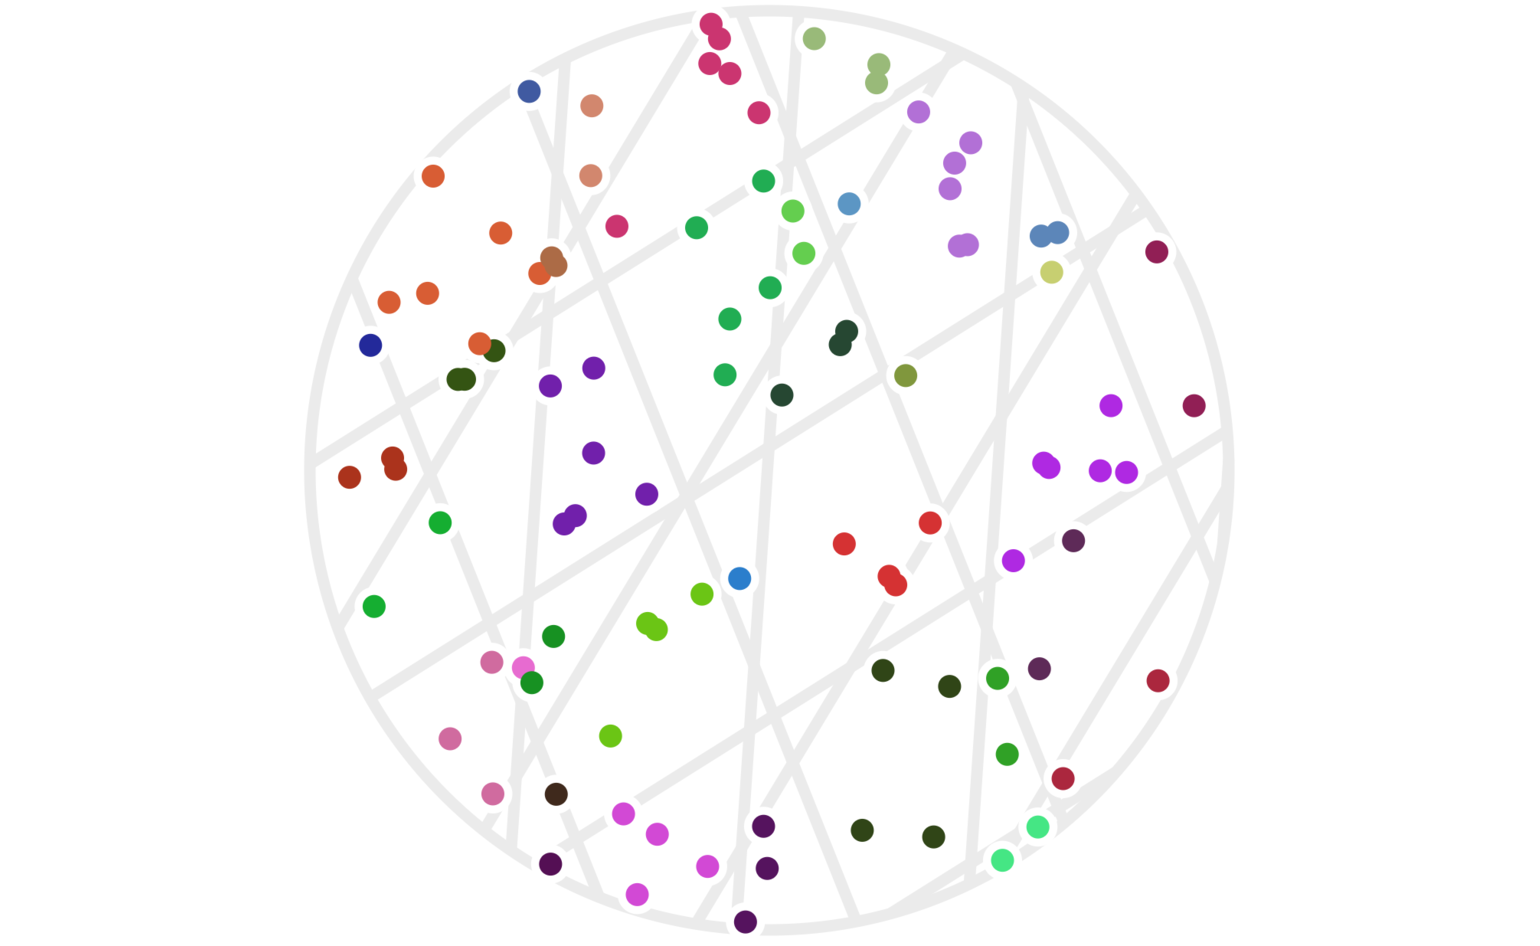
\includegraphics{images/lsh_image4.png}
\caption{One hundred random points clustered using four random hash
functions as defined by (\ref{eq:eq3}). Points have the same color when
all four of their hash values are the same. Each set of parallel light
gray lines delineates the regions with the same hash value for each of
the \(h_i()\) functions.}\label{fig:fig4}
\end{figure}

It's not obvious that we actually want to use all four of our hash
functions. The issue is that our clusters have become quite small. There
are a couple ways to address this. One is to simply increase the scale
of the hash functions; for example, set:

\[ \tilde h_i(x) := h_i(x/s), \]

where \(s\) is a scale factor. In this setup, larger \(s\) values will
result in larger clusters.

However, there is something a bit more nuanced we can look at, which is
to allow some adaptability in terms of \emph{how many hash collisions we
require}. In other words, suppose we have \(k\) total hash functions
(just above, we had \(k=4\)). Instead of insisting that all \(k\) hash
values must match before we say two points are in the same cluster, we
could look at cases where some number \(j \le k\) of them matches. To
state this mathematically, we would rewrite equation (\ref{eq:eq1}) as

\begin{equation} a \sim b \iff \#\{i: h_i(a) = h_i(b)\} \ge j. \label{eq:eq2}\end{equation}

Something interesting happens here, which is that the \(a \sim b\)
relationship is no longer a clustering, but becomes more like adjacency
(that is, sharing an edge) in a graph. The difference is that, in a
clustering, if \(a\sim b\) and \(b\sim c,\) the we must have \(a\sim c\)
as well; this is called being \emph{transitively closed}. Graphs don't
need to have this property, and in our case as well, it's no longer true
that our similarity relationship \(a\sim b\) is transitively closed.

It may help your intuition to see this new definition of \(a\sim b\) in
action on the same 100 points from figure~\ref{fig:fig4}. This time, in
figure~\ref{fig:fig5}, there are twenty random hashes, and we're seeing
the graphs generated by (\ref{eq:eq2}) using cutoff values (values of
\(j\)) of 6, 7, 8, and 9. The top-left graph in figure~\ref{fig:fig5}
has an edge drawn between two points \(a\) and \(b\) whenever there are
at least 6 hash functions \(h_i()\) with \(h_i(a) = h_i(b),\) out of a
possible 20 used hash functions.

\begin{figure}
\centering
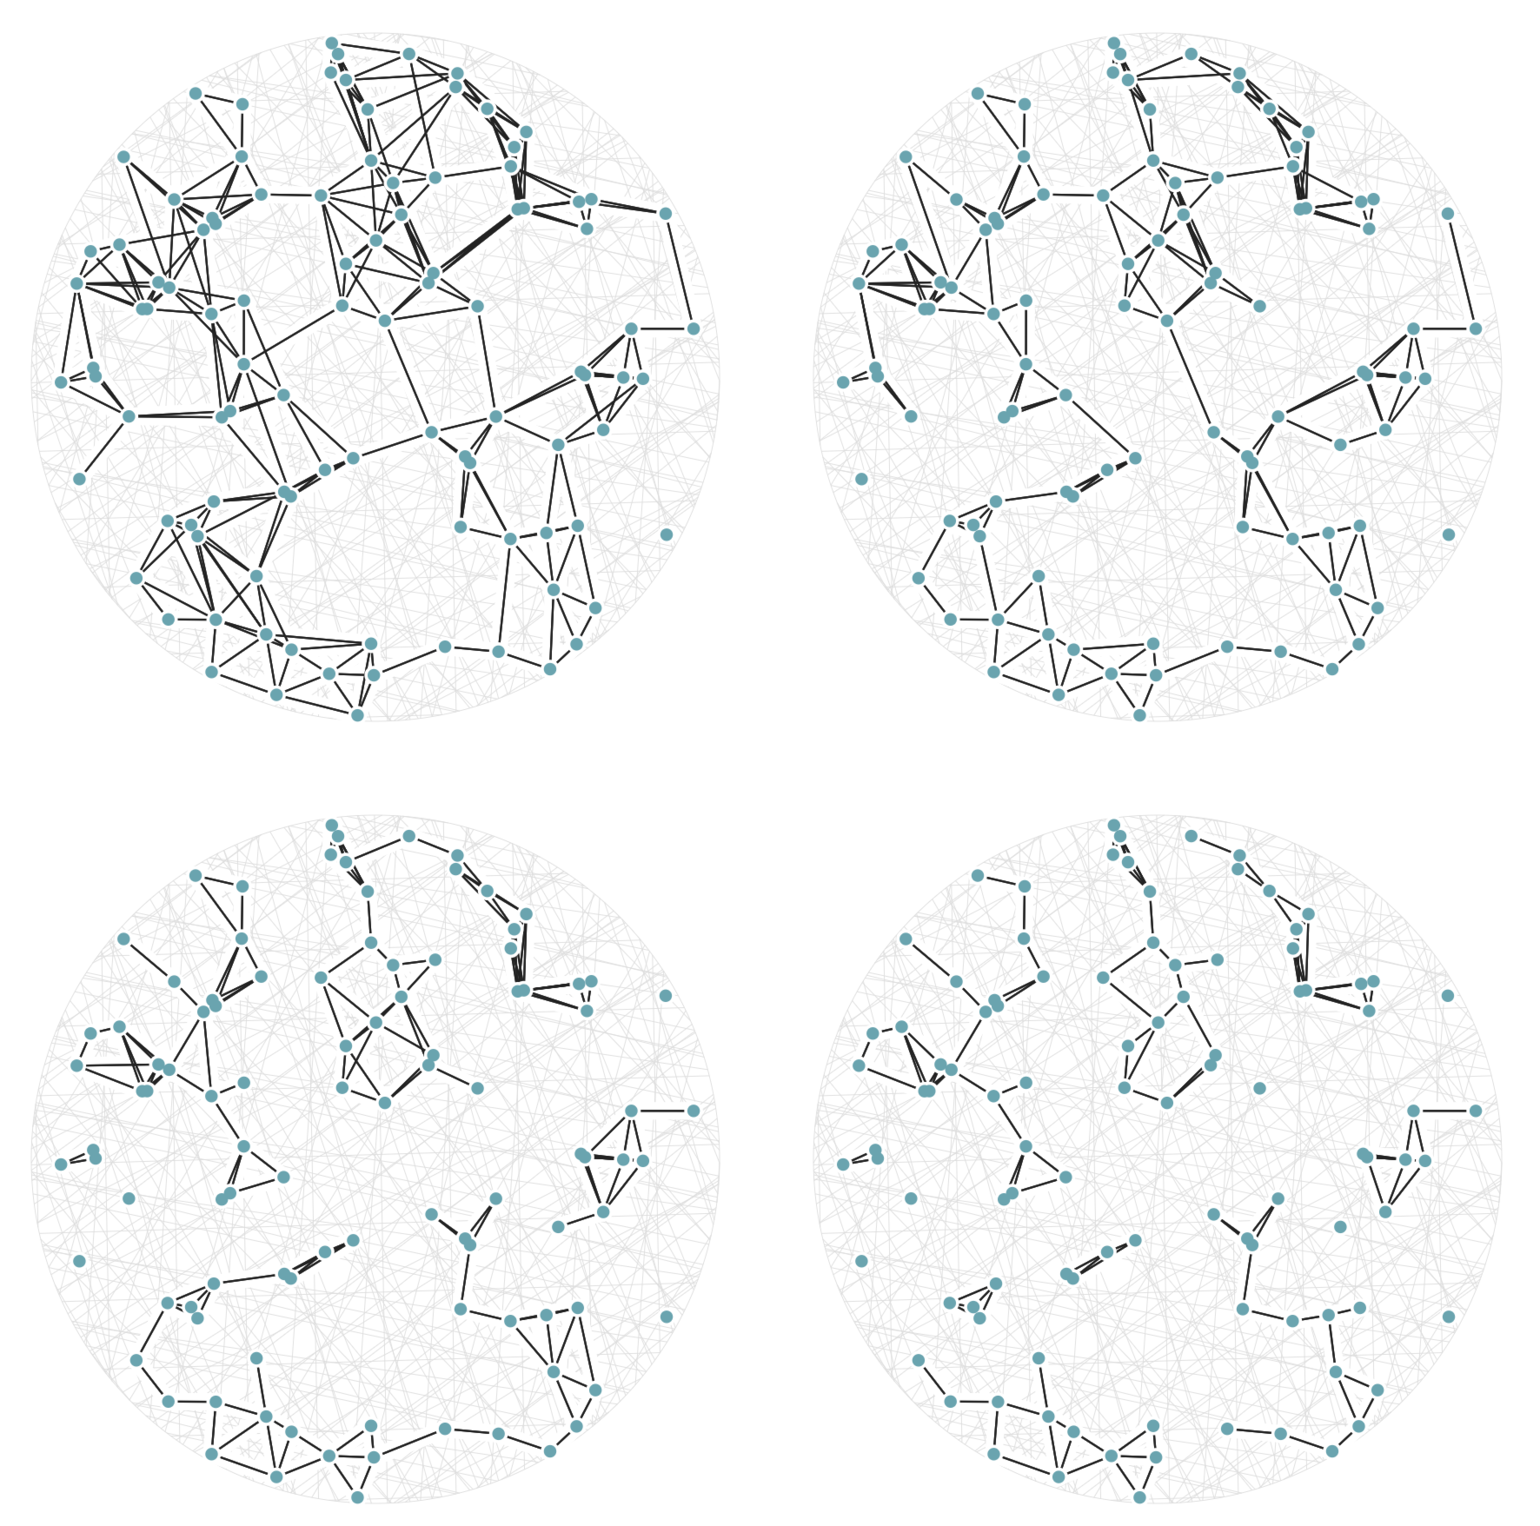
\includegraphics{images/lsh_image5.png}
\caption{A set of 100 random points with graph edges drawn according to
(\ref{eq:eq2}). There are 20 random hash functions used. The top-left
graph uses the cutoff value \(j=6.\) The remaining three graphs have
cutoff values \(j=7,\) 8, and 9; this means each graph is a subgraph
(having a subset of the edges) of the previous one.}\label{fig:fig5}
\end{figure}

In fact, we can visualize all possible cutoff values of 6 or higher ---
these are values of \(j\) in equation (\ref{eq:eq2}) --- using a single
image with weighted edges, as seen in figure~\ref{fig:fig6}.

\begin{figure}
\centering
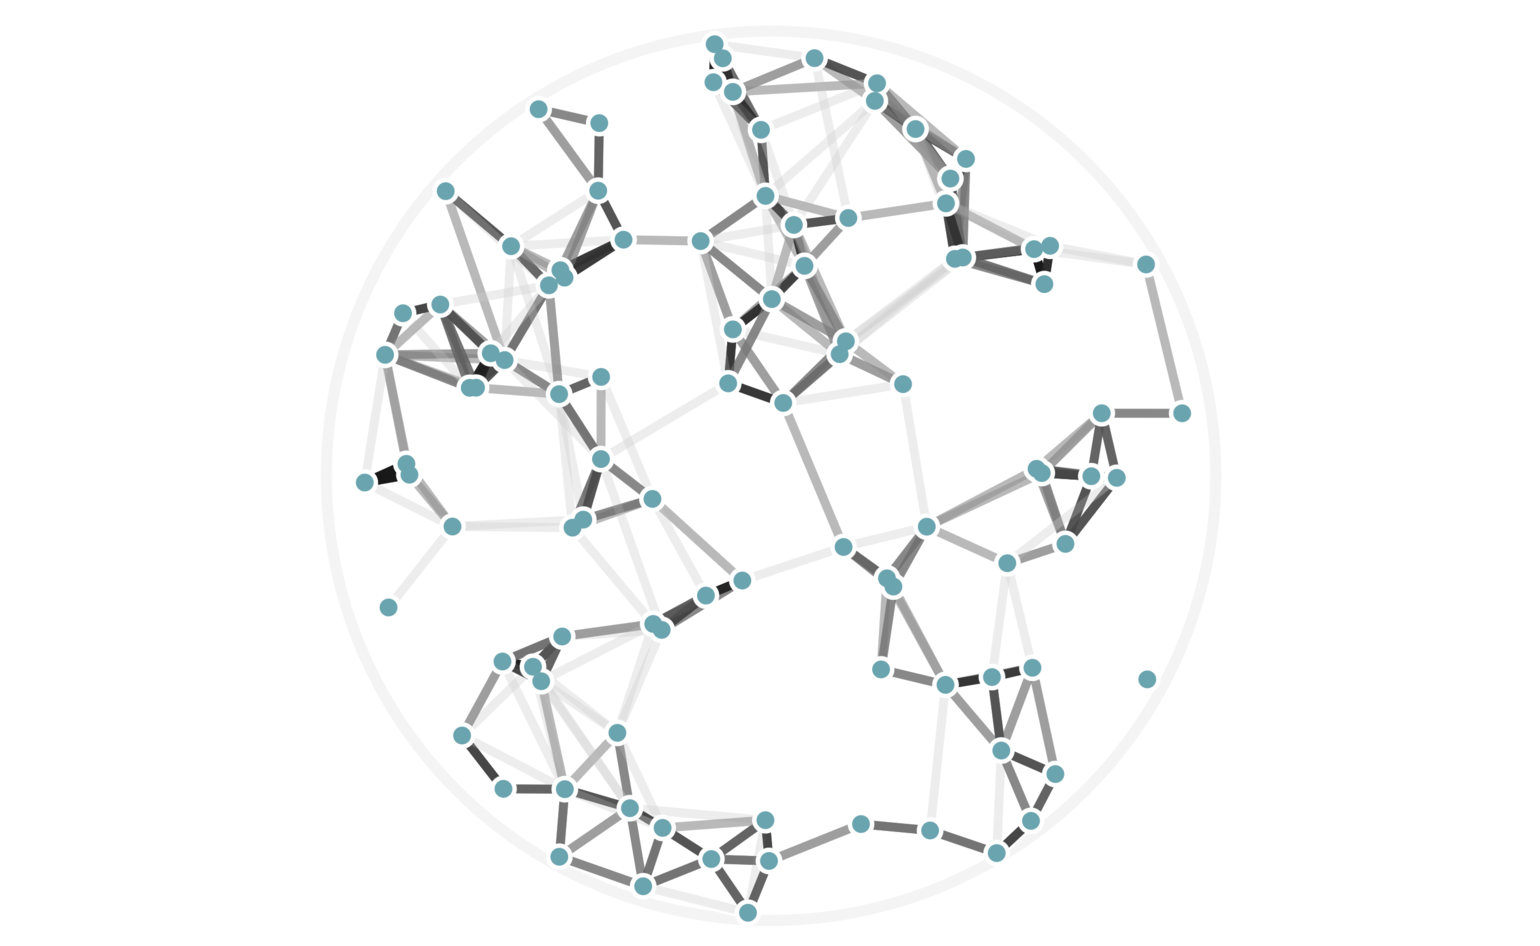
\includegraphics{images/lsh_image6.png}
\caption{The same 100 random points from figure~\ref{fig:fig5}, this
time rendered with edge weights that depend on how many hash collisions
are present between any two points. A black edge represents the maximum
of 20 hash collisions; the lightest edge represents only 6 hash
collisions.}\label{fig:fig6}
\end{figure}

There's another fun way to build intuition for what information our
hashes provide. Let's see which regions of our circle are matched, and
to what degree, by a given point. We can do this by shading regions of
the circle that will match a query point, as in figure~\ref{fig:fig8a}.
Every point in each shaded region has the same hash values for all the
hash functions used. The first part of figure~\ref{fig:fig8a} shows a
scaled version of the two-hash system (using \(h_1()\) and \(h_2()\),
similar to figure~\ref{fig:fig3}) that we saw before; the second part
uses 5 random hashes. Call the moving query point \(q;\) then any point
\(p\) in a darkly shaded region will have a hash collision
\(h_i(p) = h_i(q)\) for all hash functions; in a lightly shaded region
that equation will only hold true for a smaller subset of the hash
functions \(h_i().\)

Imagine that we were drawing these same images for some theoretically
perfect LSH setup that somehow managed to match point \(q\) to every
point \(p\) with \(||p-q||\le r\) for some radius \(r\); all other
points were not matched. For that perfect LSH setup, images like
figure~\ref{fig:fig8a} would show a fixed-size circle with center at
\(q\) that moved along with \(q\). With that in mind as the perfect LSH
result, notice that the second setting in figure~\ref{fig:fig8a} is much
closer to this ideal than the first setting. Keep in mind that lookups
within the shaded regions are no longer linear searches through data,
but rather the intersection of \(k\) hash table lookups --- that is,
lookups of nearby points are significantly faster.

\begin{figure}
\centering
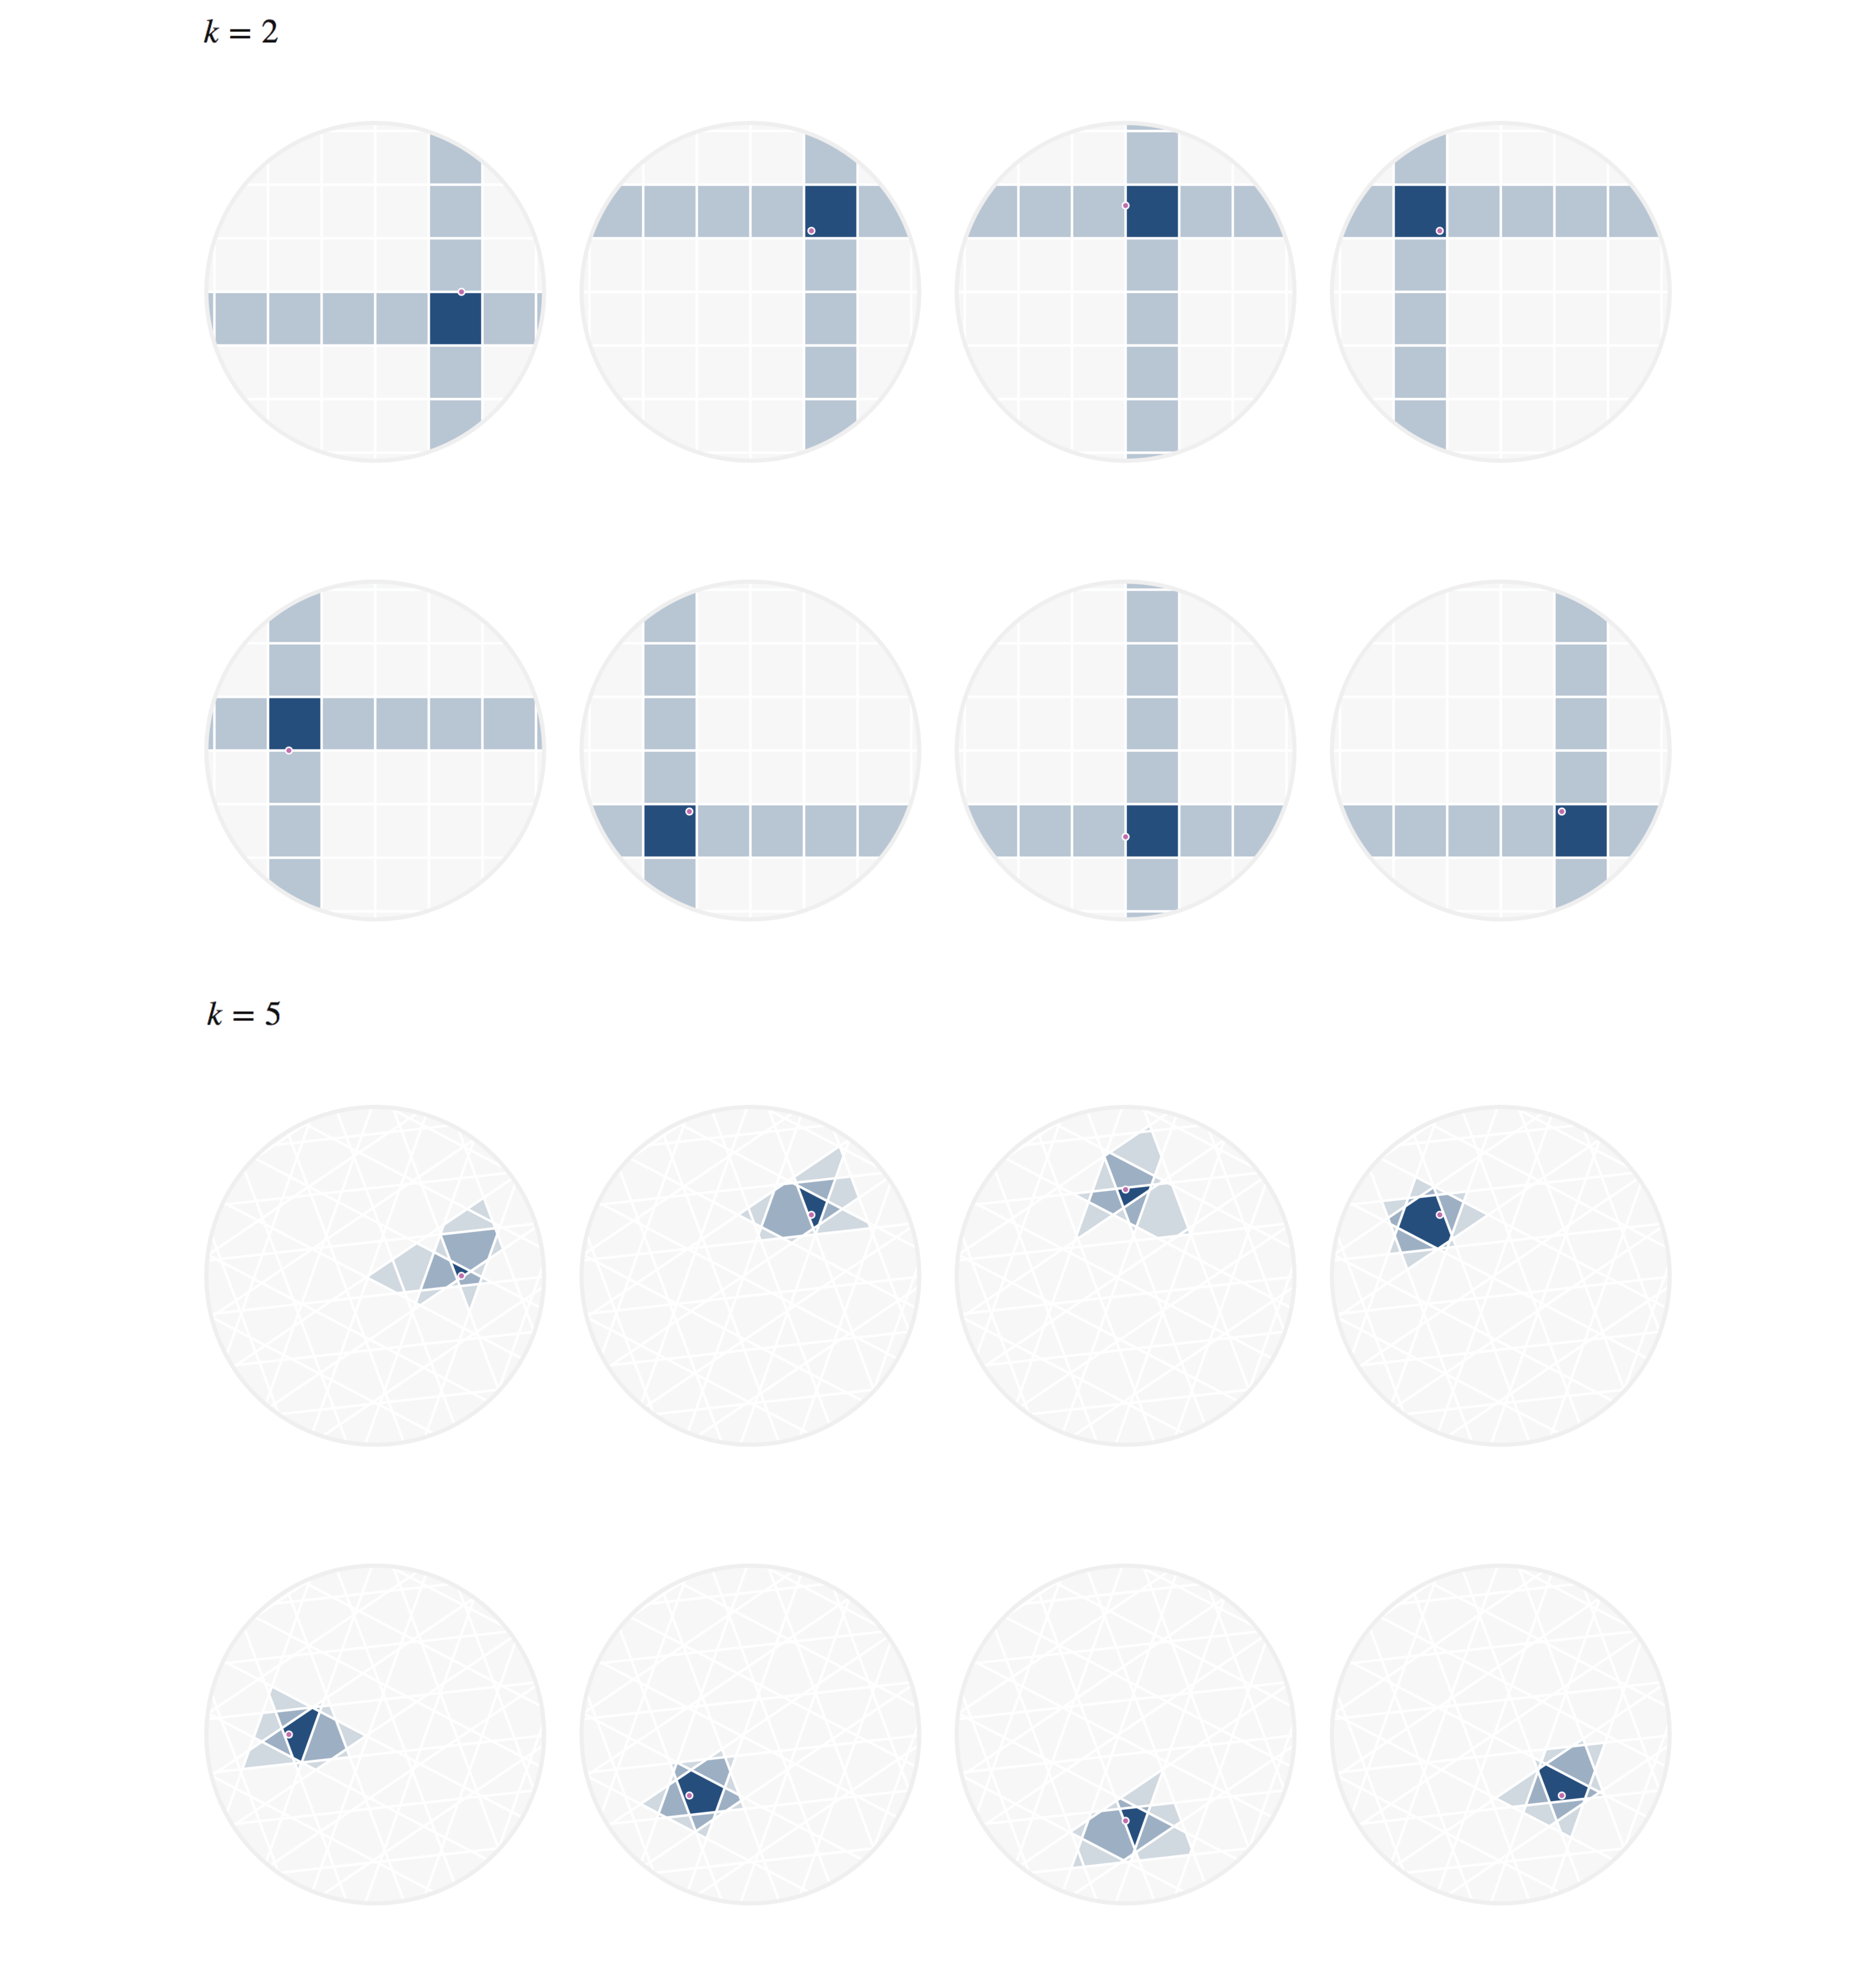
\includegraphics{images/image8a_fixed.png}
\caption{The first setting shows the regions where points would be
matched by either two (dark regions) or just one (lighter shade) hash
collision with the moving query point \(q\). The second setting shows
the analogous idea for 5 random hash functions; in the latter case, the
lightest shaded region indicates 3 hash collisions.}\label{fig:fig8a}
\end{figure}

It may further help your intuition to see how similarity edges, like
those in figure~\ref{fig:fig6}, change as a single query point moives.
This is the idea behind figure~\ref{fig:fig8b}, where weighted edges are
drawn between a moving query point and 100 random points. Notice that
the edge weightings make intuitive sense: they tend to connect strongly
to very close neighbors, weakly to farther neighbors, and not at all to
points beyond a certain distance.

\begin{figure}
\centering
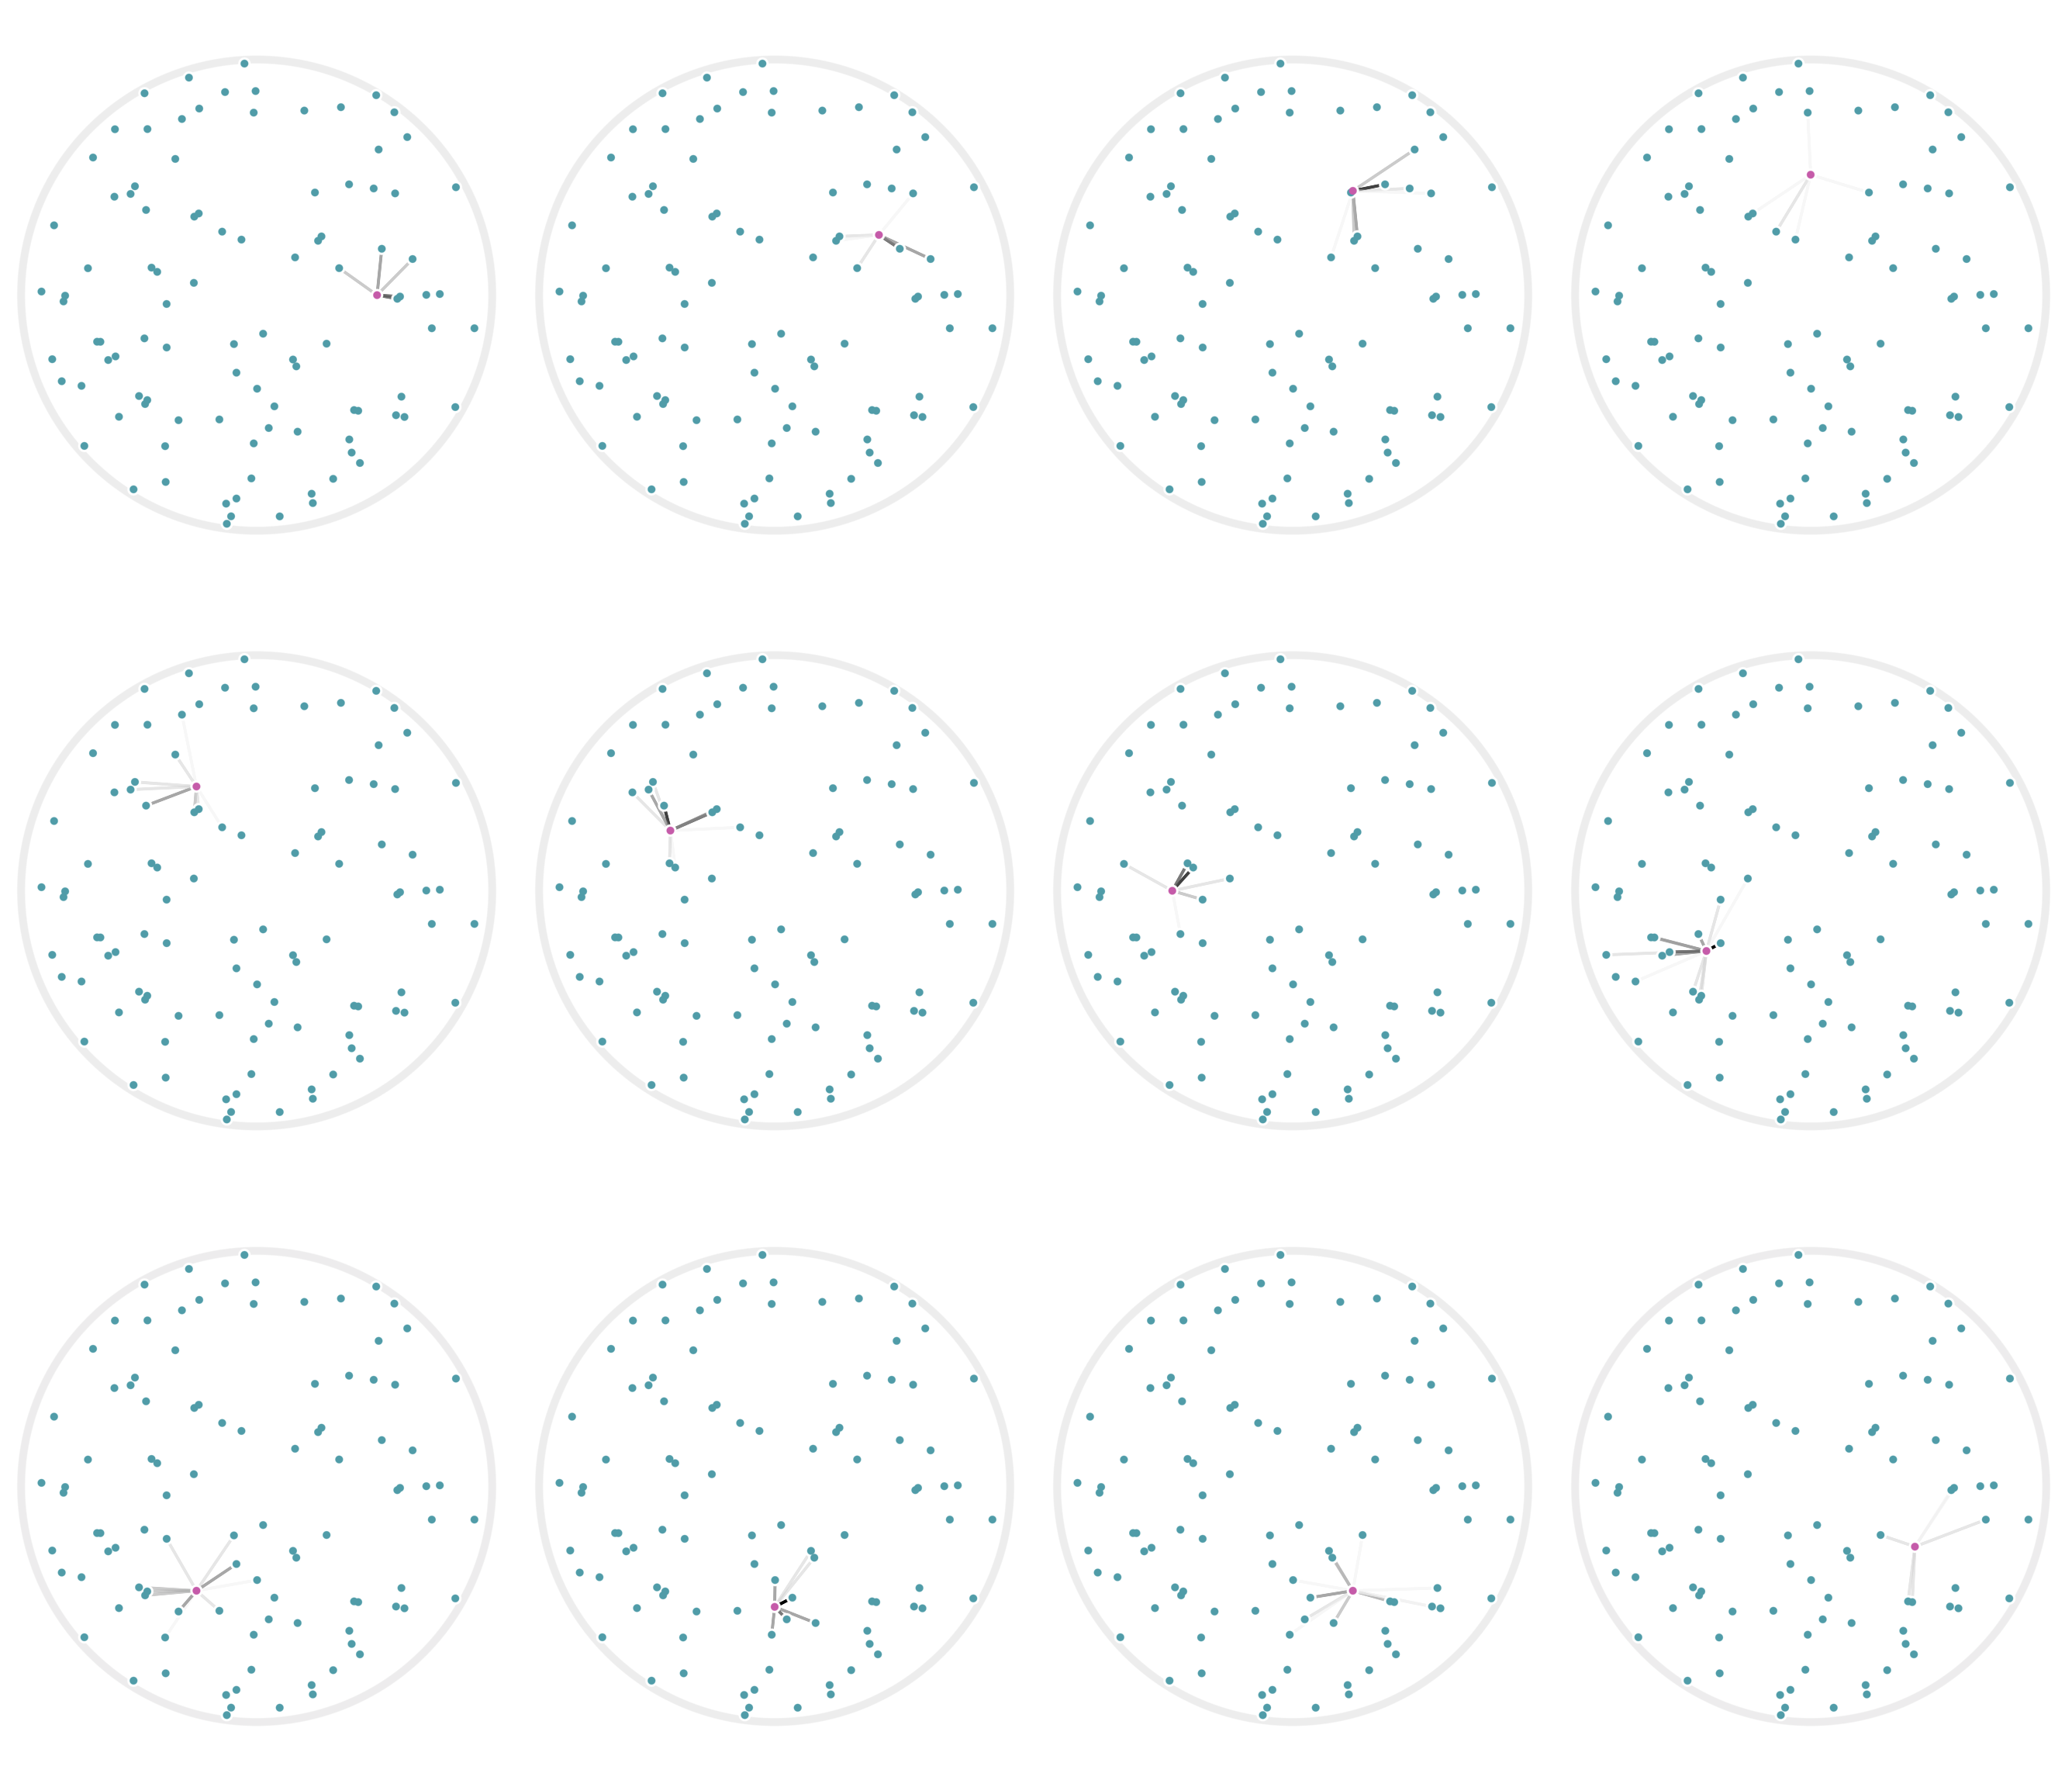
\includegraphics{images/image8b_fixed.png}
\caption{Edges weighted by how many hash collisions are present between
the moving query point and 100 random points. Darker edges indicate more
hash collisions. This image uses 12 random hashes, and requires at least
6 hash collisions for an edge to appear.}\label{fig:fig8b}
\end{figure}

\subsection{\texorpdfstring{Choosing values of
\(j\)}{Choosing values of j}}\label{choosing-values-of-j}

So far, we've seen that we can use hash lookups to find nearby neighbors
of a query point, and that using \(k\) different randomized hash
functions gives us much more accurate lookups than if we used a single
hash function. An interesting property of figure~\ref{fig:fig6} and
figure~\ref{fig:fig8b} is that we used different numbers of hash
collisions --- via the variable \(j\) --- to discover different degrees
of similarity between points. In many applications, such as findin near
duplicates or close geospatial points, we only want a binary output, so
we have to choose a particular value for \(j\). This section provides
more insight into this question of choosing good values for \(j\).

Suppose \(k\) is fixed. How can we decide which value of \(j\) is best?

To answer this question, let's temporarily consider what a perfect
function would do for us. We'll call this function \texttt{search(q)}.
In an ideal world this function returns all points within a fixed
distance of the query point. We could visualize this as an
\(n-\)dimensional sphere around the query point \(q\). A call to
\texttt{search(q)} ought to return all the indexed points \(p\) that
live within this sphere.

Let's move from that idealized algorithm into our fast-but-approximate
world of locality-sensitive hashes. With this approach, there is no
exact cutoff distance, although we keep the property that nearby
neighbors are very likely to be in the returned list and distant points
are very likely to be excluded. Since our hash functions are randomized,
we can think of the neighbor relationship \(p\sim q\) as being a
\emph{random variable} that has a certain probability of being true or
false once all our parameters are fixed (as a reminder, our main
parameters are \(j\) and \(k\)).

Now consider what great performance looks like in the context of this
random variable. Ideally, there is some distance \(D\) such that

\[||p-q|| < D-\varepsilon \quad\Rightarrow\quad P(p\sim q) > 1 - \delta;\]
\[||p-q|| > D+\varepsilon \quad\Rightarrow\quad P(p\sim q) < \delta.\]

In other words, this distance \(D\) acts like a cutoff for our
approximate search function. Points closer than distance \(D\) to query
point \(q\) are returned, while points farther are not.

I wrote a Python script to calculate some of these probabilities for the
particular parameters \(k=2\) and \(d=2\) (\(d\) is the dimensionality
of the points), and for various values of \(j\). In particular, I
restricted my input points to certain distances and measured the
probability that they had at least \(j\) hash collisions for different
\(j\) values. If you're familiar with conditional probabilities, then
this value can be written as:

\[ P\big(p \sim_j q \, \big| \, ||p-q|| = D\big), \]

where I've written \(p\sim_j q\) to denote that points \(p\) and \(q\)
have at least \(j\) hash collisions.

Using this Python script, I've visualized the collision behavior of
\(p\sim_j q\) for various \(j\) in figure~\ref{fig:fig9}. I'll go into
more detail about what each tick on the box plot indicates, but the
intuition is that shorter box plots are better because in this
visualization a shorter box plot indicates a smaller range of
uncertainty.

\begin{figure}
\centering
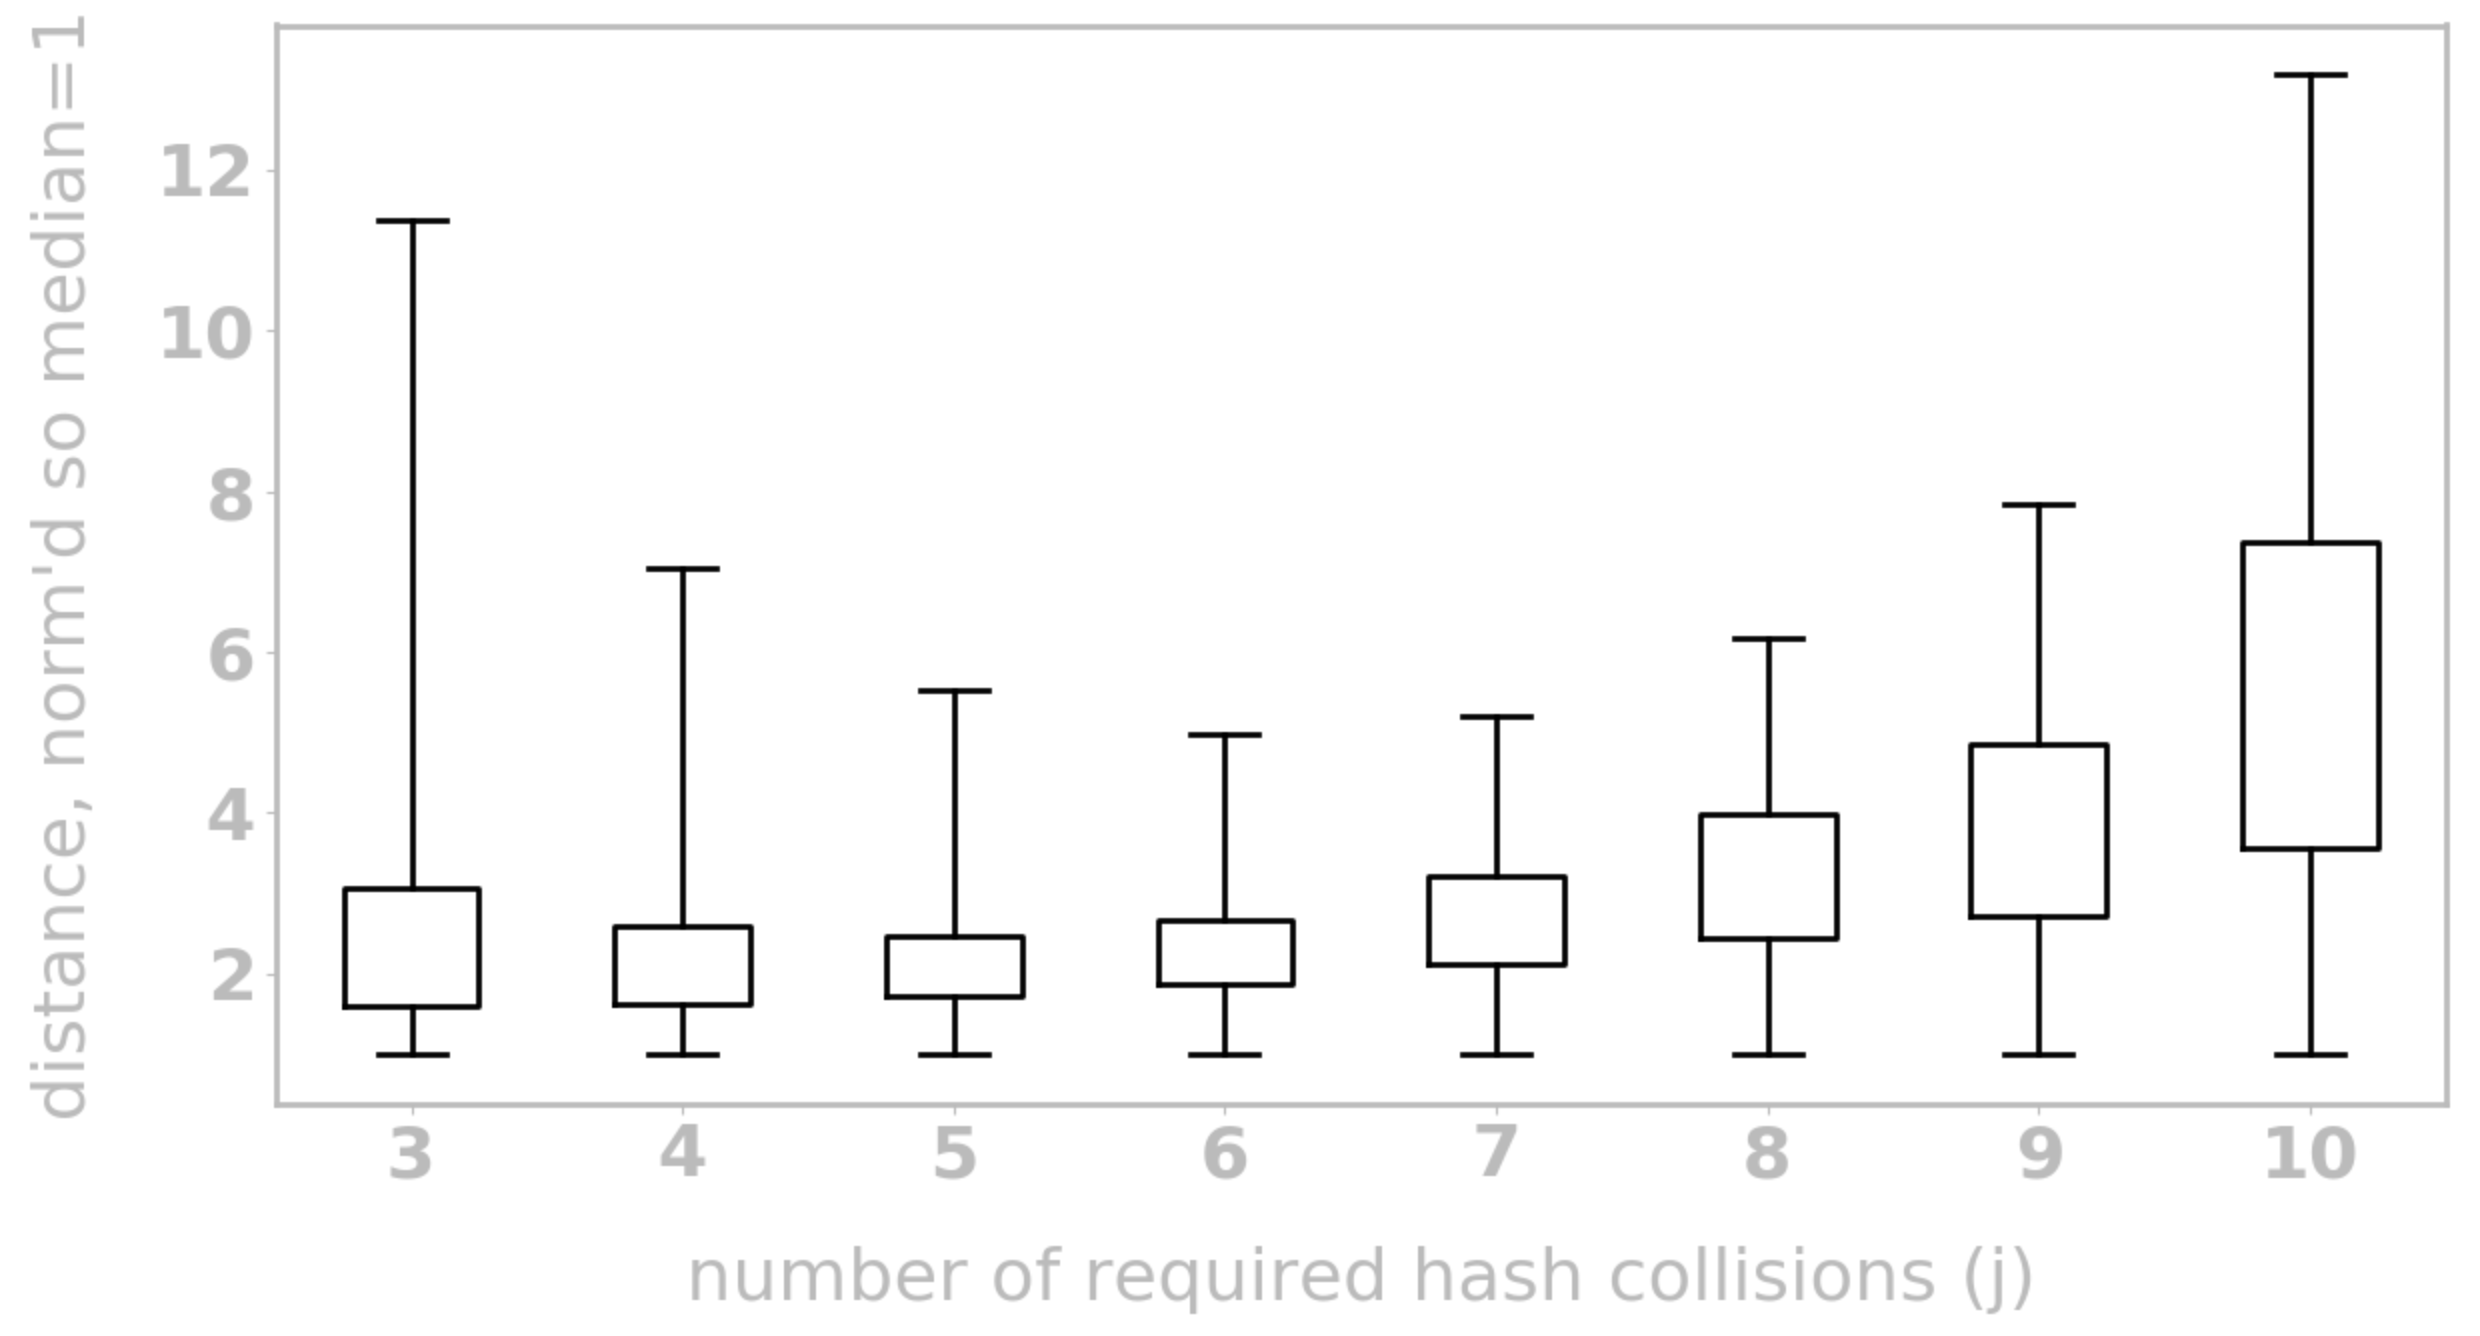
\includegraphics{images/image9@2x.png}
\caption{Intuitively, each box plot represents the distances at which
points \(p, q\) will achieve mixed results (sometimes classified as
nearby, other times as not) from our LSH setup. A very short box plot is
ideal because it indicates a smaller range of uncertainty. In other
words, a short box plot corresponds to a setting in which most pairs of
points are correctly classified by an LSH system as nearby or far apart
based on their actual distance.}\label{fig:fig9}
\end{figure}

The most interesting element of this graph is that the best value of
\(j\) appears to be \(j=6.\) You might have guessed that your best LSH
approach is to insist that \emph{all} of your random hashes must collide
before you consider two points to be neighbors, but this measurement
shows that intuition to be false.

Next I'll explain exactly what is measured in figure~\ref{fig:fig9}. A
traditional box plot visualizes the 25th and 75th percentiles of a set
of scalar data points as the boundaries of the box. Often the median
(50th percentile) is also shown within the box, but we don't include an
analogous mark in figure~\ref{fig:fig9}. The ``whiskers'' at either end
may indicate the minimum and maximum values, or something similar such
as the extreme values after removing outliers.

In our case, we have one box plot for each value of \(j\), and each plot
has been normalized so that the bottom whiskers all align at value 1.
I'll explain why this is useful in a moment. The bottom whisker
indicates the distance between \(p\) and \(q\) so that \(p\sim_j q\) is
true 99\% of the time. The bottom of the box is the relative distance at
which \(p\sim_j q\) is true 75\% of the time. Continuing in this
pattern, the box top corresponds to the distance at which we get
collisions 25\% of the time, and the top whisker is the distance at
which we get collisions 1\% of the time. Since the box plots are all
normalized (meaning that the distances per \(j\) value have all been
divided through by the smallest distance), it's easy to visually see the
ratio of each box plot position versus its smallest distance. In other
words, it's easy to visually see which distance range is smallest.

Because I love math and precision, I'm going to provide one last
definition to formalize the idea of this figure. Given a value
\(s \in (0, 1)\), define the distance \(D_s\) as the value satisfying
the given equation:

\[ P\big(p \sim_j q \, \big| \, ||p-q|| = D_s\big) = s, \]

where \(p\sim_j q\) means that \(\#\{i : h_i(p) = h_i(q)\} \ge j.\)
Intuitively, if \(\varepsilon\) is close to zero, then the distance
\(D_\varepsilon\) is large because the probability of \(p\sim_j q\) is
small. The value of \(D_{1/2}\) is just the perfect distance so that
\(p \sim_j q\) happens half of the time, and \(D_{1-\varepsilon}\) is a
small distance where \(p \sim_j q\) happens almost all the time. Using
this definition, the four values shown in each box plot of
figure~\ref{fig:fig9}, from bottom to top, are:

\[D_{.99} / D_{.99} ,\;\;
D_{.75} / D_{.99}   ,\;\;
D_{.25} / D_{.99}   ,\;\;
D_{.01} / D_{.99}.\]

\subsection{Why an LSH is faster}\label{why-an-lsh-is-faster}

So far we've been sticking to 2-dimensional data because that's easier
to visualize in an article. However, if you think about computing 10
hashes for every 2-dimensional point in order to find neighbors, it may
feel like you're doing more work than the simple solution of a linear
search through your points. Let's review cases where using an LSH is
more efficient than other methods of finding nearby points.

There are two ways an LSH can speed things up: by helping you deal with
a huge number of points, or by helping you deal with points in a
high-dimensional space such as image or video data.

\subsubsection{An LSH is fast over many
points}\label{an-lsh-is-fast-over-many-points}

If you want to find all points close to a query point \(q,\) you could
execute a full linear search. A single-hash LSH can give you results in
constant time. That's faster.

Things are slightly more complex for higher values of \(j\) and \(k.\)
If you keep \(j=k,\) then your LSH result is a simple intersection of
\(k\) different lists, each list being the set of hash collision points
returned by a given randomized hash function \(h_i().\) Finding this
intersection can be sped up by starting with the smallest of these lists
and shrinking it by throwing out points not present in the other lists.
This throwing-out process can be done quickly by using hash-table
lookups to test for inclusion in the point lists, which are basically
constant time. The running time of this approach is essentially
\(O(mk),\) where \(m\) is the length of the shortest list returned by
any of your hash functions \(h_i().\) This running time is very likely
to be an order of magnitude faster than linear search.

\subsubsection{An LSH is faster for high-dimensional
points}\label{an-lsh-is-faster-for-high-dimensional-points}

There is a beautiful mathematical result called the
\href{https://en.wikipedia.org/wiki/Johnson\%E2\%80\%93Lindenstrauss_lemma}{Johnson-Lindenstrauss
lemma} which shows that random projections (which is what we're using in
our \(h_i()\) functions) are amazingly good at preserving point-wise
distances (Dasgupta and Gupta 2003). As a result of this, you can often
use a much \emph{smaller} number of hash functions than your
dimensionality \(d\) to set up an effective LSH system.

In particular, if you have \(n\) points, then you can use on the order
of \(\log(n)\) hash functions and still achieve good results. With the
\(j=k\) approach from the last section, a lookup would require
\(O(m\log(n))\) time, where \(m\) is the length of the smallest list
returned by your hash functions. Even if you wanted to take the more
complex approach of setting \(j < k,\) you would still gain a speedup
even on pairwise comparisons. Normally it requires \(O(d)\) time to
compute the distance between two points. Using \(k \approx \log(n)\)
hashes, it would take \(O(\log(n))\) time instead to compute the number
of hash collisions between two points.

To show how significant this last speedup can be, imagine looking for
copyright violations among movie files that are 1GB each. There have
been about 500,000 movies made in the United States so far. With these
numbers, we would require looking at 2 billion numeric values of data to
directly compare two video files, versus looking at about 210 numeric
values of data to compare their LSH values. (The value 210 is twice the
expression \(8\log(500,000),\) which is a simplified suggested value for
\(k\) from the Johnson-Lindenstrauss lemma.) The LSH approach here is
about 10 million times faster.

\section{Other data types and
approaches}\label{other-data-types-and-approaches}

This article has focused on numeric, 2-dimensional data because it's
easier to visualize. Locality-sensitive hashes can certainly be used for
many data types including strings, sets, or high-dimensional vectors.

Yet another ingredient to throw into the mix here is a set of techniques
to boost performance which treat an LSH as a black box. My favorite
approach here is to simply perform multiple lookups on a hash system,
each time using \(q + \varepsilon\) as an input, where \(q\) is your
query value, and \(\varepsilon\) is a random variable centered at zero
(Panigrahy 2006).

There's a lot more that can be said about LSH techniques. If there is
reader interest, I may write a follow-up article explaining the details
of min-wise hashing, which is a fun case that's simultaneously good at
quickly finding nearby sets as well as nearby strings (Broder et al.
2000).

\begin{center}\rule{0.5\linewidth}{\linethickness}\end{center}

\section*{References}\label{references}
\addcontentsline{toc}{section}{References}

\hypertarget{refs}{}
\hypertarget{ref-broder2000min}{}
Broder, Andrei Z, Moses Charikar, Alan M Frieze, and Michael
Mitzenmacher. 2000. ``Min-Wise Independent Permutations.'' \emph{Journal
of Computer and System Sciences} 60 (3). Elsevier: 630--59.

\hypertarget{ref-dasgupta2003elementary}{}
Dasgupta, Sanjoy, and Anupam Gupta. 2003. ``An Elementary Proof of a
Theorem of Johnson and Lindenstrauss.'' \emph{Random Structures \&
Algorithms} 22 (1). Wiley Online Library: 60--65.

\hypertarget{ref-panigrahy2006entropy}{}
Panigrahy, Rina. 2006. ``Entropy Based Nearest Neighbor Search in High
Dimensions.'' In \emph{Proceedings of the Seventeenth Annual Acm-Siam
Symposium on Discrete Algorithm}, 1186--95. Society for Industrial;
Applied Mathematics.

\end{document}
